\section{Design}

Whereas recent work views user threads as a fundamental language abstraction that can
be used to implement preemptible functions, we argue just the opposite.  As discussed
in Section~\ref{sec:intro}, we believe there are already a number of clear use cases
for preemptible functions in their own right, many of which are unrelated to
parallelism and therefore have no need for the scheduler, multiple kernel threads, or
synchronization to support a full threading abstraction.  To prove that our
abstraction does not compromise on expressive power, we end this section by
demonstrating how it can be trivially applied to convert an existing cooperative
userland threading library to a preemptive one.

\begin{figure}
\begin{verbatim}
struct linger {
  bool is_completion;
  union {
    void *completion;
    opaque_t continuation;
  };
};

typedef void *(*function_t)(void *);

struct linger launch(function_t func,
  uint64_t time);
  void *args);
void resume(struct linger *timed_func,
  uint64_t time);
\end{verbatim}
\caption{Core libinger (C language) interface}
\label{fig:interface}
\end{figure}

We propose an interface consisting of two functions, \texttt{launch()} and
\texttt{resume()} (Figure~\ref{fig:interface}).  Both are ordinary, structured calls
whose invocation adheres to C's standard stack discipline; there is no
continuation-style or unstructured control flow.  Client code creates a preemptible
function by passing an ordinary function (or closure) to the \texttt{launch()}
function along with an execution time cap (in microseconds).  If the function
completes on time, \texttt{launch()} propagates its result to the caller; otherwise,
it returns an opaque continuation object that the caller may later pass to
\texttt{resume()} to continue executing the function from wherever it was preempted.
Figure~\ref{fig:usage} shows a basic usage example where the caller is obligated to
perform some work after a certain amount of time (say, call a watchdog), but first
calls into some helper code with weak time bounds.  Thanks to preemptible functions,
the caller doesn't have to trust the helper to know that the watchdog will be called
in time.

\begin{figure}
\begin{verbatim}
res = launch(helper, TIMEOUT, NULL);
call_watchdog(); // Won't be delayed.
if(res.is_completion)
  // We're already done.
  return res.completion;
else
  // Give helper() some more time.
  resume(&res, TIMEOUT);
// ...
\end{verbatim}
\caption{Basic libinger usage example}
\label{fig:usage}
\end{figure}

Although the interface we propose bears some similarities to that of Scheme
engines~\cite{haynes:iucs1984}, some of our design decisions deliberately differ from
theirs:  (1) We return a structured type instead of a function, since the latter
approach would be unportable between languages.  Note that in languages with operator
overloading, it's possible to achieve the other syntax by defining the
\texttt{linger} type's function-call operator to call the \texttt{resume()} function.
(2) Because the preemptible function itself may state, we make the \texttt{linger}
type stateful as well, allowing \texttt{resume()} to mutate it in place.
(3) Instead of passing the preemptible function's return value to a separate callback
function, we return it directly from \texttt{launch()}.  This decision was made
because many modern languages have first-class tagged union (sum) types that allow
the compiler to enforce that the caller explicitly checks whether the function
completed and only accesses the appropriate side of the union.  In addition to the
barebones C interface, our current implementation provides a Rust interface
demonstrating many of these extensions.

Those familiar with futures may notice their applicability to preemptible functions
and simularity to our interface.  While each language's futures differ slightly,
preemptible function bindings can be constructed in the following trivial manner:
To create a new preemptible future, the bindings should call \texttt{launch()} with a
budget of 0 $\mu$s.  Each attempt to poll the future for a value should resolve to a
call to \texttt{resume()} with the timeout passed to poll (if allowed by the
language's API), or else previously associated with the future by other means.

The rest of this section describes the implementation of a novel open-source software
stack supporting preemptible functions and fine-grained userland preemptive
threading.  We start by discussing \textit{libgotcha} (Section~\ref{sec:libgotcha}),
a library that seeks to automatically address many problems related to shared state
in third-party code.  Next, we give an aside illustrating the straightforward
application of libgotcha to provide POSIX async-signal-safety in places where it
wouldn't otherwise exist (Section~\ref{sec:statefulness}).  We then cover the
\textit{libinger} library for running preemptible functions
(Section~\ref{sec:libinger}) and its interaction with libgotcha.  Finally, we present
our experience with porting a userland threading library to libinger in order to make
it preemptive (Section~\ref{sec:threading}).  Figure~\ref{fig:architecture} shows
these components in the overall architecture.

\begin{figure}
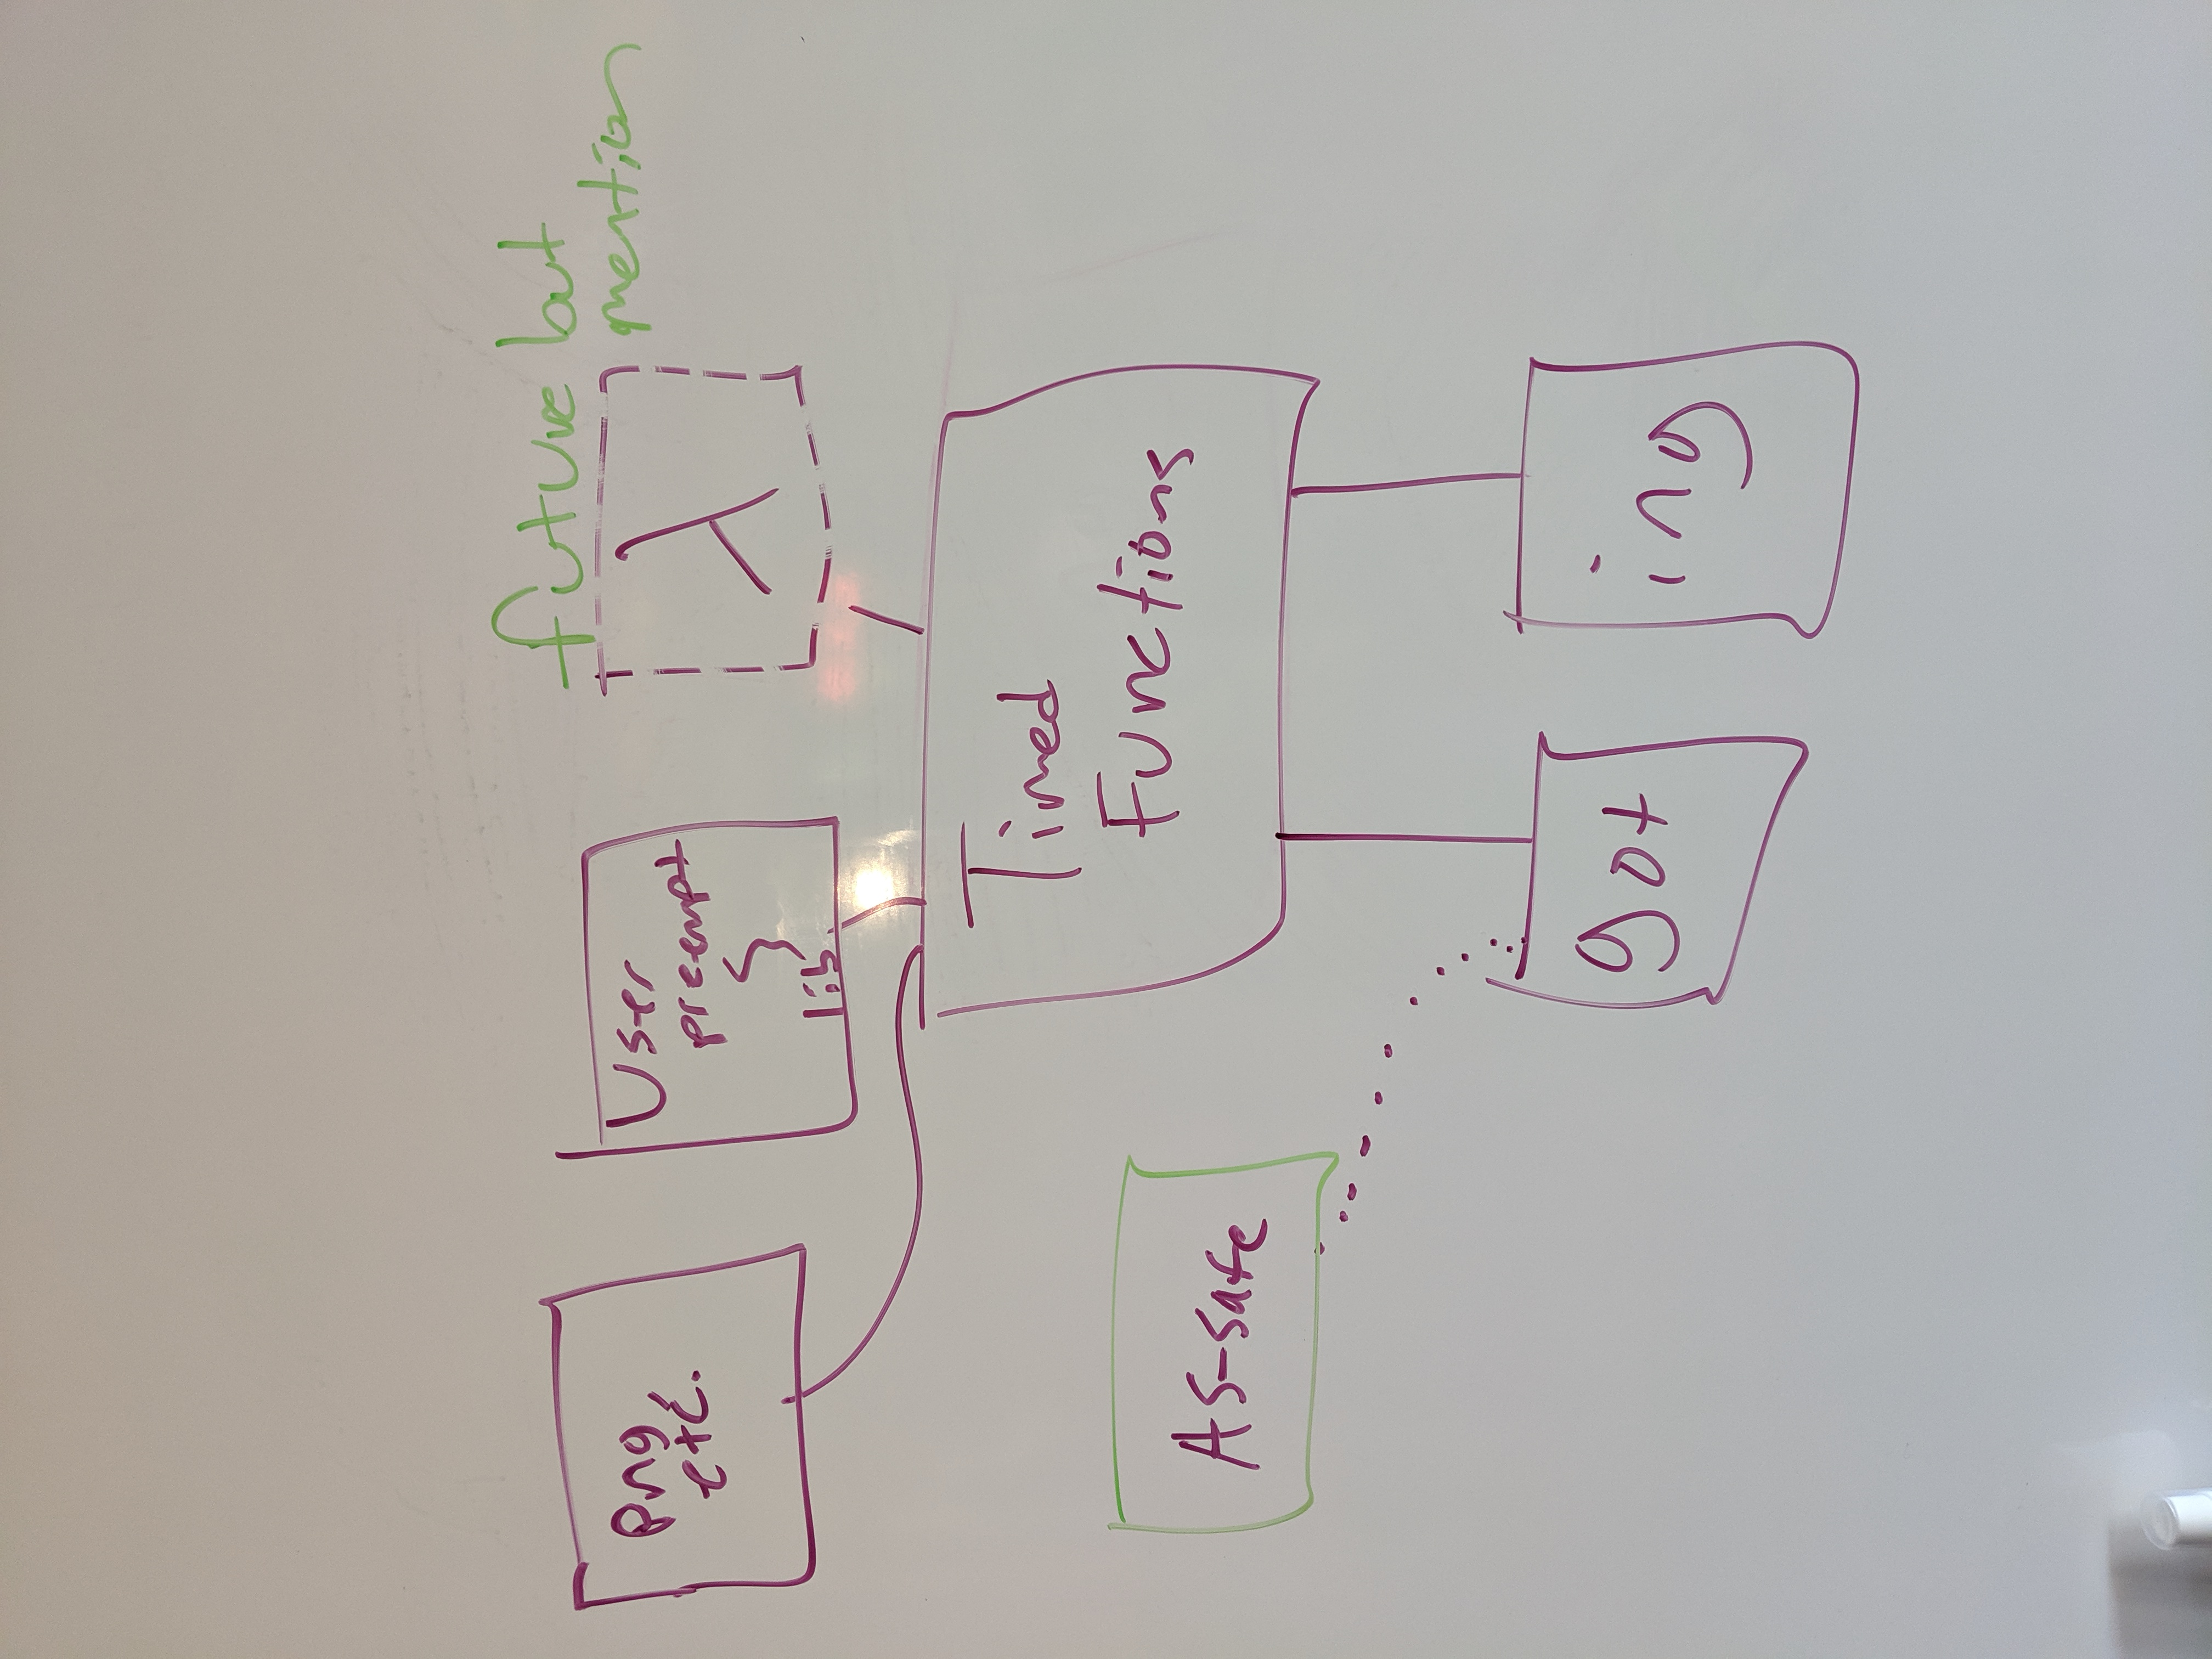
\includegraphics[height=\columnwidth,angle=270]{figs/architecture}
\caption{Architecture of preemptible functions stack}
\label{fig:architecture}
\end{figure}

\subsection{Shared state: \textit{libgotcha}}
\label{sec:libgotcha}

Although shared state is always a problem for preemptible functions, we classify code
that relies on shared state depending on its location:\@ we term it \textbf{internal
stateful code} if it is part of a project (i.e., in the same linked object file)
that uses preemptible functions, and \textbf{external stateful code} otherwise (e.g.,
as is the case for third-party libraries).  Recall that one of our goals is to
support third-party libraries without needing to recompile them.

We begin by briefly discussing internal stateful code.  Figure~\ref{fig:bug} shows
a code passage with a concurrency bug:\@ because the \texttt{timed()} function does
not use an atomic increment operation, its \texttt{launch()} invocation might be
preempted after reading the \texttt{count} variable but before writing it, in which
case the \texttt{resume()} will preserve the existing value of \texttt{1}, causing
the assertion to fail.  We take the stance that internal stateful code is responsible
for implementing its own concurrency control to fix this kind of problem, since the
developers are aware they are using preemptible functions, and therefore (hopefully)
are also aware of the concurrency implications.  If the internal stateful code is
written in Rust instead of C, the compiler can statically prevent many such bugs by
forcing the user to use atomics or locks to protect shared variables such as
\texttt{count}.

\begin{figure}
\begin{verbatim}
static int count = 0;

static void *timed(void *ignored) {
  ++count;
}

int main(void) {
  struct linger res =
    launch(timed, VERY_SHORT, NULL);
  ++count;
  resume(&res, LONG_ENOUGH);
  assert(count == 2); // BUG!

  return 0;
}
\end{verbatim}
\caption{Concurrency bug in internal stateful code}
\label{fig:bug}
\end{figure}

The problem we do have to handle is external stateful code, since there's no way an
existing piece of code can be expected to know that it might be called from a
preemptible function.  In other words, the developers of libraries such as
\texttt{libc} should not need to know that preemptible functions exist.  On the other
hand, we cannot restrict programs that use preemptible functions to calling only
async-signal-safe functions.  This is where libgotcha comes in:\@ it instruments the
boundaries between relocated ELF object files (i.e., executables and dynamic shared
objects), which we term \textbf{cross-library references} (in the case of global
variables) and \textbf{cross-library calls} (in the case of function calls).

\solb{May need to explicitly define these as a subset of dynamic .*s}

To accomplish both objectives, we slightly weaken the guarantees of either dynamic
linking or preemption, depending on the scenario.  In the common case, we weaken the
property that every use of a dynamically-linked function or global variable resolves
to the same address:\@ we open multiple copies of the shared objects required by the
application, and direct cross-library references to a separate copy for each
preemptible function.  In this way, we ensure that inconsistent state from a library
used by one preemptible function cannot affect uses of that same library by other
preemptible functions or the broader application.  While this approach works for many
libraries, it is sometimes inappropriate; for instance, using multiple copies of the
dynamic allocator would cause them to manage the same heap with different free lists.
In such cases, we direct all dynamic calls to the same copy of the function and defer
preemption on that thread until the call has completed, in the style of goroutines.
The rest of this section describes the implementation of these two approaches.  Note
that, in principle, libgotcha functions with the unmodified GNU dynamic linker.

\paragraph{GOTs and PLTs}

When a dynamically-linked executable is run, the kernel first passes control to the
dynamic linker, \texttt{ld.so}, which loads all required shared object files and
populates their respective \textbf{global offset tables (GOTs)}\footnote{It is from
these structures that \textit{lib\textbf{got}cha} gets its name.} with the resolved
addresses of any referenced dynamic symbols.  Once the program is loaded, any
dynamic references to global variables (which correspond to x86-64 instructions of
the form \texttt{mov~\textit{symbol}@gotpcrel(\%rip),~\%\textit{dest}}) look up the
target symbols' addresses in the GOT for the object file containing the referencing
code.

Dynamic function calls are slightly more complicated because they can resolve lazily
the first time they are called.  For instance, the instruction
\texttt{call~printf@plt} causes the assembler to generate a corresponding executable
\textbf{Procedure Linkage Table (PLT)} stub function, as shown in
Figure~\ref{fig:plt}.  The first instruction of this stub looks up the address of the
function by checking a corresponding GOT entry; however, initially this contains the
address of the immediately-following \texttt{pushq} instruction!  Thus, on the first
call, the PLT stub pushes a symbol relocation identifier (here, \texttt{0x0}) onto
the stack and calls into the dynamic linker, which resolves the symbol to the
function's real address, memoizes the result by updating the GOT entry, and finally
jumps into the real function.  Subsequent calls to the PLT stub then forward to the
real function after executing only the initial \texttt{jmpq} instruction.

\begin{figure}
\begin{verbatim}
0000000000001030 <printf@plt>:
  1030:  jmpq   *0x2fe2(%rip) <printf>
  1036:  pushq  $0x0
  103b:  jmpq   1020 <.plt>
\end{verbatim}
\caption{Example PLT entry for call to \texttt{printf()}}
\label{fig:plt}
\end{figure}

\subsection{Case study: Establishing AS-safety}
\label{sec:statefulness}

\subsection{Preemptible functions: \textit{libinger}}
\label{sec:libinger}

\subsection{Case study: Userland threading}
\label{sec:threading}

\solb{Discuss Table 1 from Shinjuku and its implications for our design}

\solb{Go ``also'' heap-allocates goroutine locals: \url{https://github.com/golang/go/issues/33216}}
